\documentclass[review]{elsarticle}
\usepackage{graphicx}
\usepackage{hyperref}

%% To allow supplementary table and figure numbering
%% http://bytesizebio.net/2013/03/11/adding-supplementary-tables-and-figures-in-latex/

\newcommand{\beginsupplement}{%
		        \setcounter{table}{0}
		        \renewcommand{\thetable}{S\arabic{table}}%
		        \setcounter{figure}{0}
		        \renewcommand{\thefigure}{S\arabic{figure}}%
			     }

\journal{Ecological Modelling}

\title{MixFishSim: Supplementary Figures and Tables}

\begin{document}

\beginsupplement
\maketitle

\begin{figure}[!ht]
	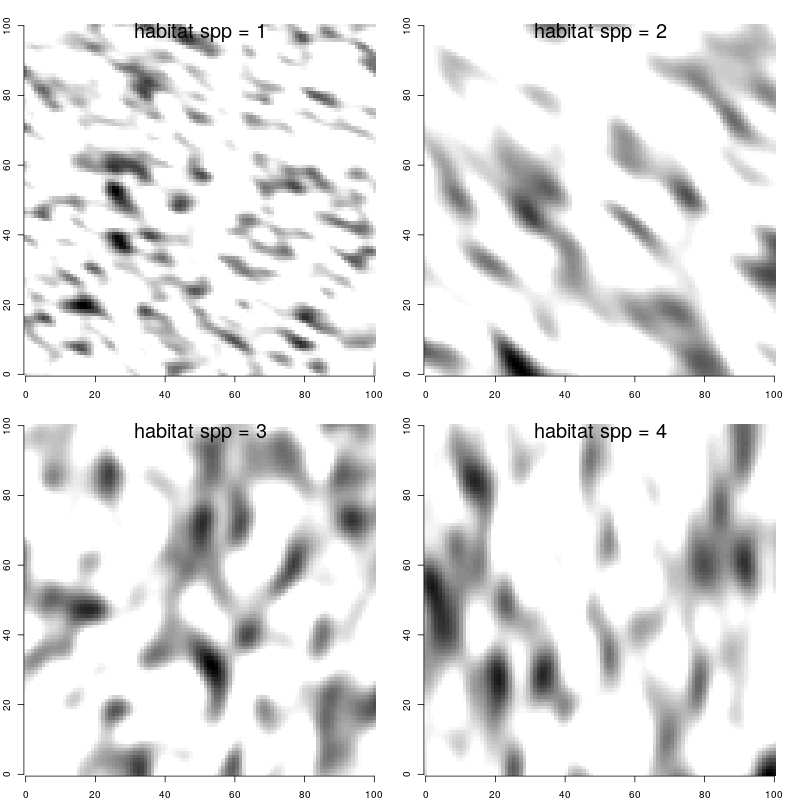
\includegraphics[width = \linewidth]{../analysis/habitat}
	\caption{habitat preference}
	\label{fig:1}
\end{figure}	

\begin{figure}[!ht]
	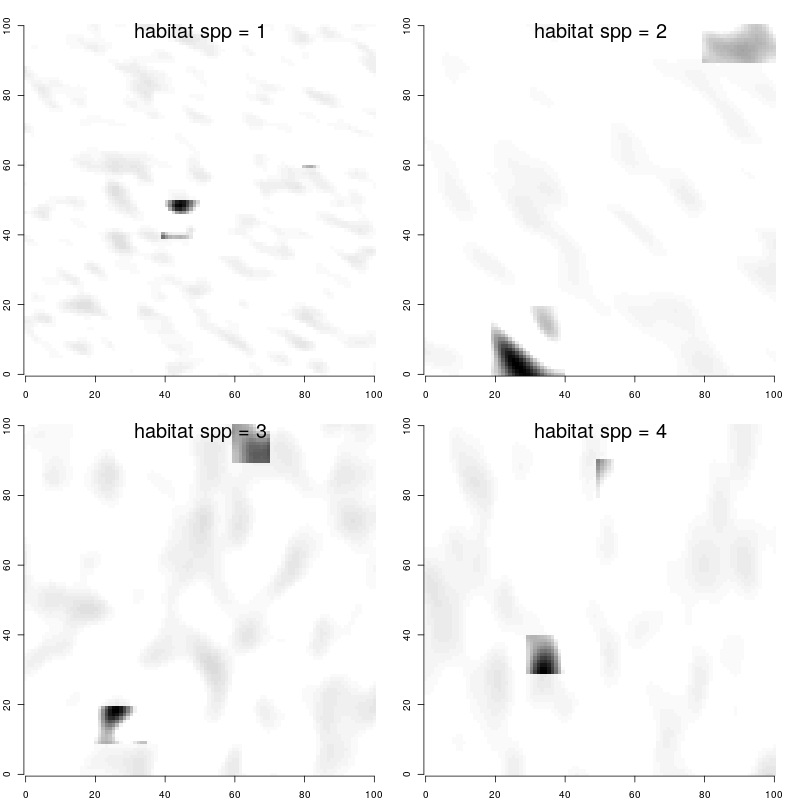
\includegraphics[width = \linewidth]{../analysis/habitat_spwn}
	\caption{spawning habitat preference}
	\label{fig:2}
\end{figure}	


\begin{figure}[!ht]
	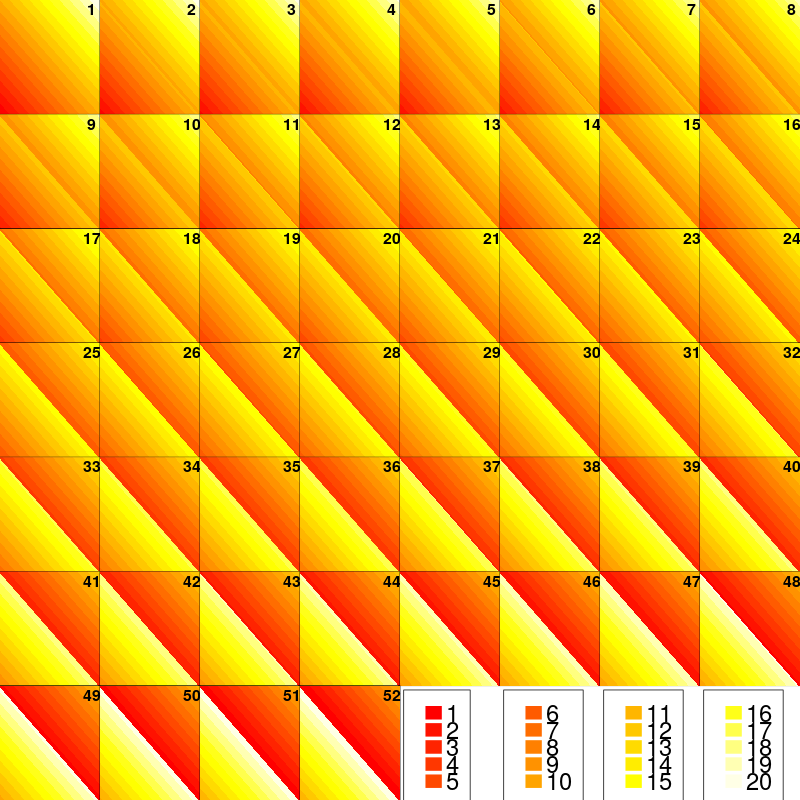
\includegraphics[width = \linewidth]{Plots/Temperature_gradient}
	\caption{Spatiotemporal temperature gradient}
	\label{fig:3}
\end{figure}

\begin{figure}[!ht]
	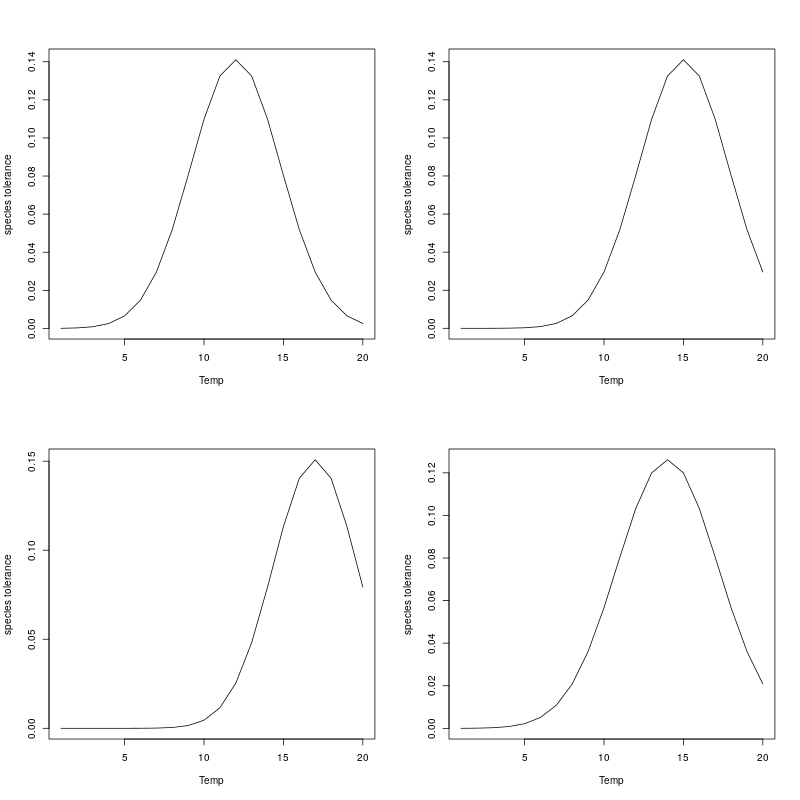
\includegraphics[width = \linewidth]{Plots/Species_tolerances}
	\caption{Species thermal tolerances}
	\label{fig:4}
\end{figure}

\begin{figure}[!ht]
	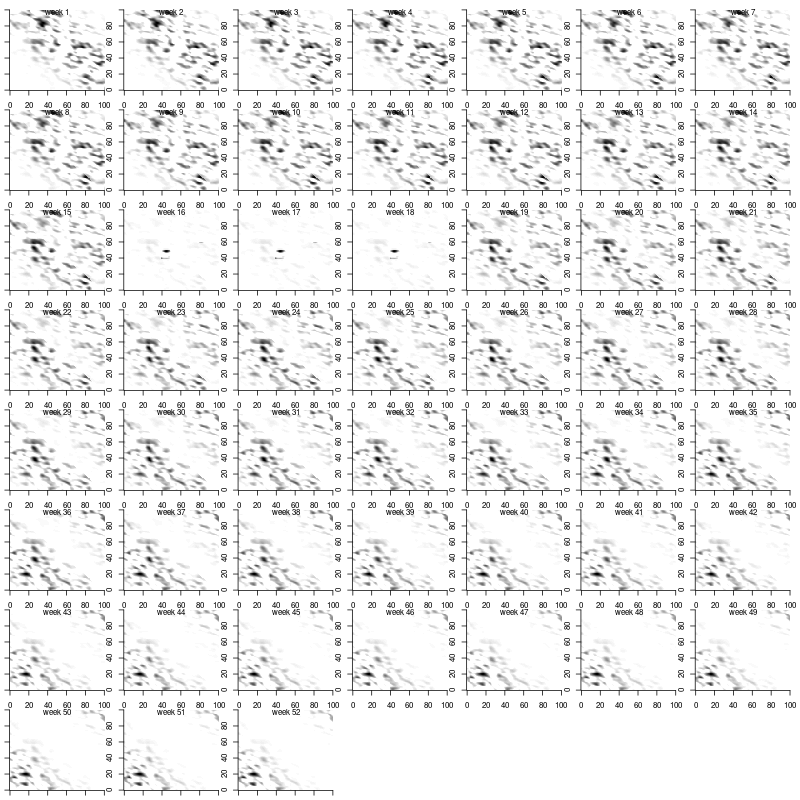
\includegraphics[width = \linewidth]{Plots/habitat_spatiotemp_spp_1}
	\caption{Spatiotemporal habitat suitability - population 1}
	\label{fig:5}
\end{figure}

\begin{figure}[!ht]
	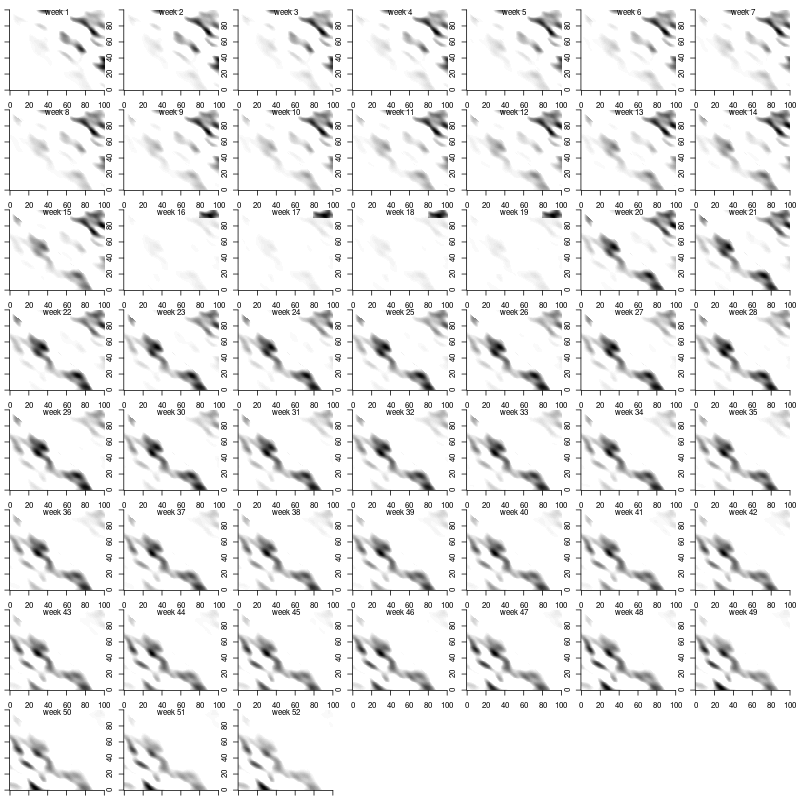
\includegraphics[width = \linewidth]{Plots/habitat_spatiotemp_spp_2}
	\caption{Spatiotemporal habitat suitability - population 2}
	\label{fig:6}
\end{figure}

\begin{figure}[!ht]
	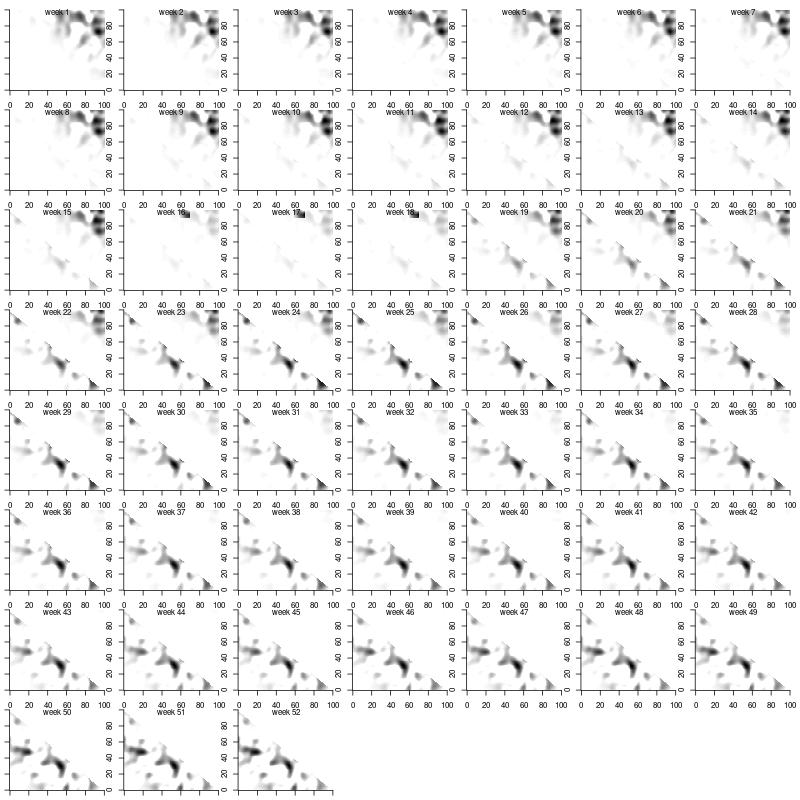
\includegraphics[width = \linewidth]{Plots/habitat_spatiotemp_spp_3}
	\caption{Spatiotemporal habitat suitability - population 3}
	\label{fig:7}
\end{figure}

\begin{figure}[!ht]
	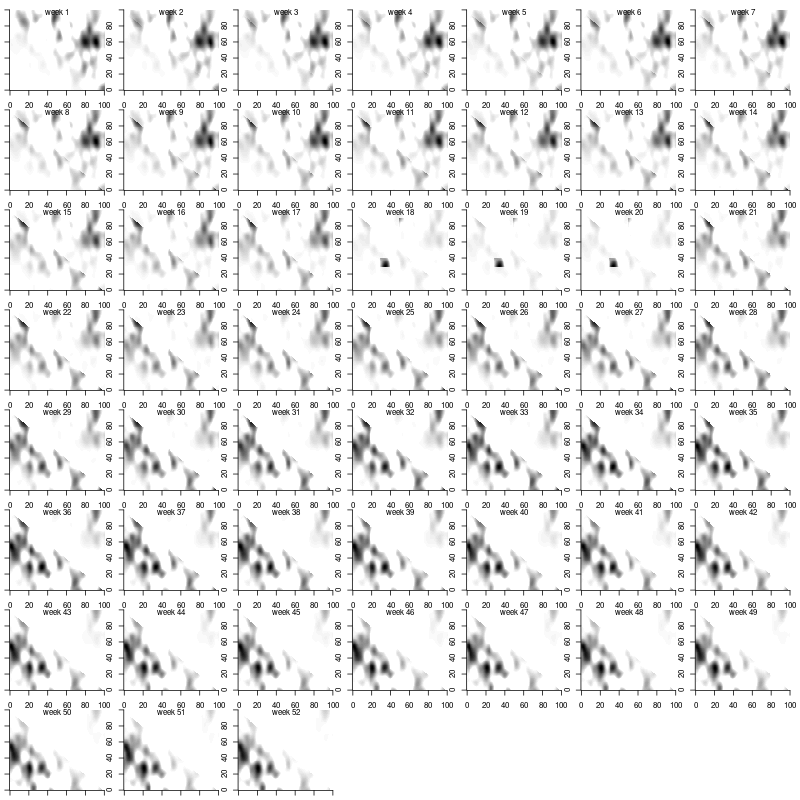
\includegraphics[width = \linewidth]{Plots/habitat_spatiotemp_spp_4}
	\caption{Spatiotemporal habitat suitability - population 4}
	\label{fig:8}
\end{figure}

\begin{figure}[!ht]
	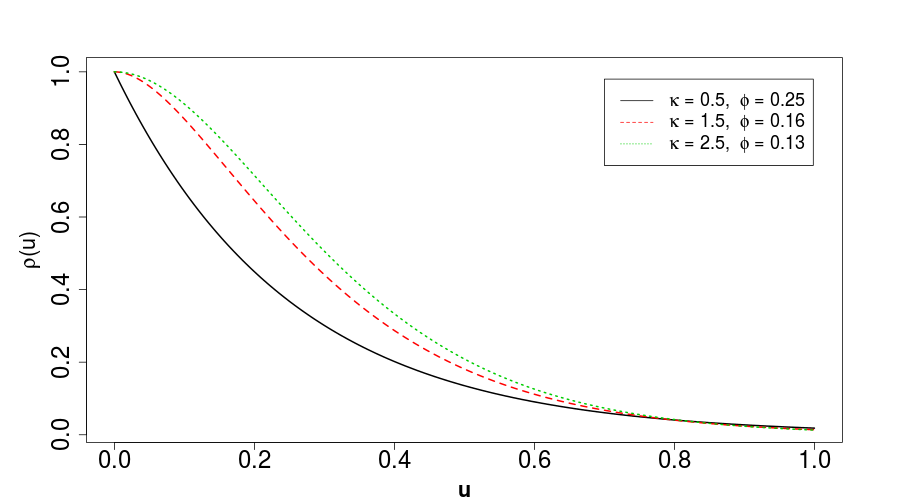
\includegraphics[width = \linewidth]{./Plots/Matern}
	\caption{Example of different implementation of the Matern correlation
	function on autocorrelation distance}
	\label{fig:16}
\end{figure}	



\end{document}

